\subsection{Lokal optimal løsning}
Når først en optimal løsning er fundet, er det nødvendigt at tjekke, at der ikke er tale om en lokal optimal løsning.
\begin{defn}[Lokalt optimal løsning]
Lad $\vec{x} \in P$ være en løsnings til et minimeringsproblem med objektfunktion $f$, da er $\vec{x}$ en \textbf{lokal optimal løsning}, hvis 
\begin{align*}
\exists \epsilon > 0, \forall \vec{y} \in P, \vec{x}\neq \vec{y} \, : \, |\vec{x}-\vec{y}| < \epsilon \Rightarrow f(\vec{x})\leq f(\vec{y}).
\end{align*}
\end{defn}
Betragt beviset for Sætning \ref{stn:eksistens}, det bygger på ideen om at lægge en retningsvektor til en vilkårlig vektor, så deres sum har en mere optimal værdi end vektoren. 
Hvis denne metode bruges til at finde en optimal løsning frem for en mulig basisløsning vil et lokalt minimum, som ikke er en optimal løsning kunne opstå, hvis der ikke eksistere en retningsvektor, men der er en løsning, hvis værdi er mere optimal, se Figur \ref{fig:lokaltmin}.
\begin{figure}
\begin{center}
	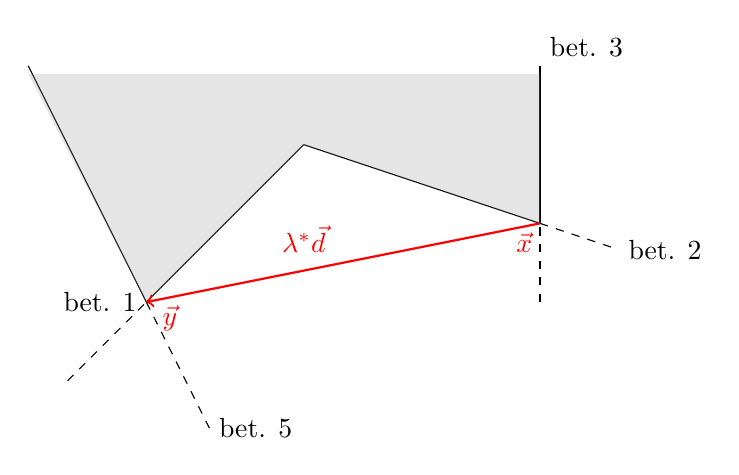
\begin{tikzpicture}[ latex
  s/.style={width=0}]

  %ligning 1
	\draw[domain=-1:0,variable=\x,dashed] 	plot({\x},{\x})  node[left] {bet. 1};
	\draw[domain=0:2,variable=\x] 			plot({\x},{\x});

	
  %ligning 2
	\draw[domain=2:5,variable=\x] 			plot({\x},{-(1/3)*\x+8/3});
	\draw[domain=5:6,variable=\x,dashed] 	plot({\x},{-(1/3)*\x+8/3}) node[right] {bet. 2};
	

  %ligning 3
	\draw[domain=0:1,variable=\y, dashed] 			plot({5},{\y});
	\draw[domain=1:3,variable=\y] 	plot({5},{\y}) node[above right] {bet. 3};
	

	
  %ligning 5
  	\draw[domain=-1.5:0,variable=\x] 	plot({\x},{-2*\x}) ;
	\draw[domain=-0:4/5,variable=\x, dashed] 			plot({\x},{-2*\x}) node[right] {bet. 5} ;


  %løsningsmængden skraveret
	\fill[gray!80,nearly transparent]  (0,0) -- (2,2) -- (5,1) -- (5,2.9) --(-1.5,2.9) --  cycle;
	
  % vektor x
  \node[thick, color=red] (x) at (4.8,0.75) {$\vec{x}$};
  
\node[thick, color=red] (y) at (0.3,-0.2) {$\vec{y}$};
%   %\node[s] (d) at (2, -0.5);
 \draw[thick, color=red, ->](5,1) -- (0,0) node[above, yshift=0.5 cm, xshift=2 cm] {$\lambda^* \vec{d}$} ;
%   \node[] (x) at (2.1, -0.6) {$\vec{x}+\lambda^* \vec{d}$};
%  % \path (x) edge node[right] {$\vec{x}+\lambda^* \vec{d}$} (d) ;
 
\end{tikzpicture}
	\captionof{figure}{Bemærk at der ikke eksistere en retningsvektor $\vec{d}$, så der kan konstueres en bedre løsning, uden at overskride betingelse $2$, derfor vil løsningsvektor $\vec{x}$ fremstå optimal, selvom at løsningsvektor $\vec{y}$ er mere optimal. Løsningsvektor $\vec{x}$ er et lokalt minimum.}
	\label{fig:lokaltmin}
\end{center}
\end{figure}
Det er dog ikke alle mængder, hvor der kan forekomme lokale optimale løsninger, som ikke også er en optimal løsning.
\begin{defn} [Konveks mængde]
Lad $S \subset \mathds{R}^n$  da er $S$ konveks, hvis der $\forall \vec{x}, \vec{y} \in S$ og et vilkårligt $\lambda \in [0,1]$ gælder, at \\ 
$\lambda \vec{x} + (1-\lambda) \vec{y} \in S$.
\label{def:Konveks}
\end{defn}
En konveks mængde er en mængde, der opfylder, at det vægtede gennemsnit af et hvert par af elementer også tilhører mængden, det betyder, at der altid kan findes en retningsvektor mellem et hvert punkt i mængden.
Helt generelt gælder det, hvis løsningsmængden til et lineært ligningsproblem er konveks, så vil en hver lokal optimal løsning være en optimal løsning.
\begin{stn}
Lad $\vec{x} \in P$ være en lokal optimal løsnings til et lineært programerignsproblem  med objektfunktion $f$.
Da er  $f(\vec{x}) \leq f(\vec{y})$ for alle $\vec{y} \in P$ hvis $P$ er konveks.
\end{stn}
\begin{proof}
Antag at $\vec{x}^* \in P$ er en optimal løsning.
Da $P$ er konveks medfører det, at $\lambda \vec{x}^* + (1-\lambda)\vec{x} \in P$. 
Da $\lambda$ kan vælges til at være vilkårligt tæt på nul, må $|(\lambda \vec{x}^* + (1-\lambda)\vec{x}) - \vec{x}| < \epsilon$ da
\begin{align*}
 |\lambda \vec{x}^* + (1-\lambda)\vec{x} - \vec{x}| = | \lambda \vec{x}^* - \lambda\vec{x}| = \lambda|\vec{x}^* - \vec{x}| < \epsilon.
\end{align*}
Da $\vec{x}$ er en lokal optimal løsning, følger det, at
\begin{align*}
f(\vec{x}) \leq f(\lambda \vec{x}^* + (1-\lambda)\vec{x}).
\end{align*}
Da $f$ er lineær følger det af Definition \ref{def:linfunk}, at 
\begin{align*}
f(\vec{x}) \leq f(\lambda \vec{x}^* + (1-\lambda)\vec{x}) &= \lambda f(\vec{x}^*) + (1-\lambda)f(\vec{x}) \qquad \Rightarrow
\\ f(\vec{x}) - f(\vec{x}) &\leq \lambda f(\vec{x}^*) + f(\vec{x})-\lambda f(\vec{x}) - f(\vec{x}) \qquad \Rightarrow
\\ 0 & \leq \lambda( f(\vec{x}^*) - f(\vec{x})),
\end{align*}
hvis $\lambda$ er lille nok.
Da $ \lambda$ kan være forskellig fra nul, og $f(\vec{x}^*)\leq f(\vec{x})$ må det medføre, at $f(\vec{x}^*) - f(\vec{x}) = 0$, hvorfor $f(\vec{x}^*) =f(\vec{x})$. 
Det kan derfor konkluderes, hvis $\vec{x}$ er en lokal optimal løsning, så er $\vec{x}$ en optimal løsning.
\end{proof}
Løsningsmængden  for et standard problem, vil altid være konveks.
\begin{stn}
Lad $P =\{ \vec{x} \in \mathds{R}^n \mid A \vec{x} \geq \vec{b}\} $ være et polyeder, da er $P$ konveks.
\label{stn:polykon}
\end{stn}
\begin{proof}
Lad $\vec{x}, \vec{y} \in P$ være to vilkårlige vektorer, da gælder, at $A\vec{x} \geq \vec{b}$, hvilket medfører, at $\lambda A \vec{x} \geq \lambda\vec{b}$, hvor $\lambda \in [0,1]$ er en skalar. 
På ligefod må der derfor gælde, at $(1-\lambda)A\vec{y} \geq (1-\lambda)\vec{b}$.
De to uligheder adderes nu
\begin{align*}
\lambda A \vec{x} + (1-\lambda) A \vec{y} \geq \lambda \vec{b} + (1 - \lambda) \vec{b}
\\  A (\lambda\vec{x} + (1-\lambda)\vec{y}) \geq \vec{b}.
\end{align*}
Derfor må $\lambda\vec{x} + (1-\lambda)\vec{y} \in P$.
\end{proof}
Det betyder derfor, at et hvert lineært programmeringsproblem kun har optimale løsninger, da det er vist i Kapitel \ref{Afsnit:LinProg}, hvordan ethvert lineært programmerings problem kan skrives på standard form.

